\chapter{概率论与分布}
\label{chap:probability}
\markboth{概率论与分布}{概率论与分布}

\begin{remark}[本章定位]\label{rem:probability_chapter_positioning}
本章系统建立概率论与分布理论的基本框架，重点讨论随机变量与分布函数、常见分布族及其相互关系、特征函数与傅里叶变换的统一、贝叶斯推断、随机过程的基本类型、以及大数定律与中心极限定理。

\textbf{与周期数学的核心接口}：概率论与周期数学在四个层面深度交汇：其一，\textbf{概率分布的特征函数就是分布的傅里叶变换}（定理 \ref{thm:characteristic_fourier}），分布的全部信息编码在特征函数的模与相位中，与周期函数的频谱分析完全同构；其二，\textbf{圆周 $S^1$ 上的均匀分布是圆群上的 Haar 测度}（定义 \ref{def:uniform_distribution}），其旋转不变性正是 $U(1)$-对称在概率层面的实现；其三，\textbf{循环群 $C_N$ 上的概率分布}（命题 \ref{prop:discrete_cyclic}）与周期序列、离散傅里叶变换、循环卷积构成完整的代数-概率对应；其四，\textbf{平稳过程与循环平稳过程}（定义 \ref{def:stationary_process}、\ref{ch14_cyclostationary}）是时间平移群在随机过程上的作用，其自协方差函数的谱分解（定义 \ref{def:power_spectral_density}）与功率谱是周期数学在随机层面的核心工具。

\textbf{本章七主题导引}：平移——平稳过程在时间平移群 $\mathbb{Z}$（离散）或 $\mathbb{R}$（连续）作用下的统计不变性（定义 \ref{def:stationary_process}），以及序贯贝叶斯更新沿时间轴的推进（定义 \ref{def:sequential_bayesian}）；缩放——自相似过程与重尾分布在标度变换 $t\mapsto\lambda t$ 下的标度不变性（Hurst 指数 $H$、尾指数 $\alpha$，定义 \ref{ch14_scale_invariance}），以及中心极限定理的标度收敛（定理 \ref{thm:central_limit_theorem}）；旋转——特征函数辐角 $\arg\phi_X(t)$ 在频率空间的相位信息（注 \ref{prop:characteristic_grammar}）、$S^1$ 上均匀分布的旋转对称（定义 \ref{def:uniform_distribution}）；守恒——自协方差在时间平移下的不变性（命题 \ref{ch14_autocovariance_stationarity}）与标度指数在标度变换下的不变性；对称——先验/似然/后验三元结构下的分布族对称（共轭先验的封闭性，定义 \ref{def:conjugate_prior}）；闭合——大数定律与中心极限定理的收敛闭合（定理 \ref{thm:weak_law_of_large_numbers}、\ref{thm:central_limit_theorem}）与遍历轨道“时间平均$=$空间平均”的闭合判据（定理 \ref{thm:birkhoff_ergodic}）；周期——循环平稳过程的周期 $T$（定义 \ref{ch14_cyclostationary}）与马尔可夫链特征值 $|\lambda_i|=1$ 的周期模式（命题 \ref{prop:transfer_operator_eigen}）。
\end{remark}

\begin{figure}[htbp]
\centering
\begin{tikzpicture}[
  font=\small,
  box/.style={draw, rounded corners, fill=blue!8, minimum width=2.6cm, minimum height=0.8cm, align=center},
  sub/.style={draw, rounded corners, fill=green!10, minimum width=2.4cm, minimum height=0.7cm, align=center, font=\footnotesize},
  arr/.style={->, thick, >=stealth}
]
  % 第一行：概率论核心
  \node[box] (prob) {概率空间\\$(\Omega,\mathcal F,\mathbb P)$};
  \node[box, right=0.8cm of prob] (rv) {随机变量\\分布函数};
  \node[box, right=0.8cm of rv] (cf) {特征函数\\傅里叶变换};
  \node[box, right=0.8cm of cf] (dist) {常见分布\\族与关系};
  % 第二行：与周期数学的接口
  \node[sub, below=1.0cm of prob] (stat) {平稳过程\\时间平移不变};
  \node[sub, below=1.0cm of rv] (cyc) {循环平稳\\周期平移不变};
  \node[sub, below=1.0cm of cf] (ss) {自相似\\标度不变};
  \node[sub, below=1.0cm of dist] (markov) {马尔可夫链\\特征值周期};
  % 第三行：统一
  \node[box, fill=orange!12, below=1.0cm of $(stat)!0.5!(markov)$] (unify) {概率论与周期数学的统一：平移/缩放/旋转/周期四条主线};
  \draw[arr] (prob) -- (rv);
  \draw[arr] (rv) -- (cf);
  \draw[arr] (cf) -- (dist);
  \draw[arr] (prob) -- (stat);
  \draw[arr] (rv) -- (cyc);
  \draw[arr] (cf) -- (ss);
  \draw[arr] (dist) -- (markov);
  \draw[arr] (stat) -- (unify);
  \draw[arr] (cyc) -- (unify);
  \draw[arr] (ss) -- (unify);
  \draw[arr] (markov) -- (unify);
\end{tikzpicture}
\caption{本章结构总览：概率论核心（概率空间、随机变量、特征函数、分布族）与周期数学接口（平稳、循环平稳、自相似、马尔可夫链），最终统一于四条主线。}
\label{fig:probability_overview}
\end{figure}

\section{事件及其概率}\label{sec:events_probability}

\subsection{随机事件与概率}

\begin{definition}[随机事件]\label{def:random_event}
在概率空间 $(\Omega, \mathcal{F}, \mathbb{P})$ 中，$\mathcal{F}$ 中的元素称为\textbf{随机事件}。事件 $A$ 的\textbf{概率} $\mathbb{P}(A)$ 是 $[0,1]$ 中的实数，满足：
\begin{enumerate}[label=(\roman*)]
    \item \textbf{非负性}：$\mathbb{P}(A) \ge 0$ 对所有 $A \in \mathcal{F}$ 成立。
    \item \textbf{规范性}：$\mathbb{P}(\Omega) = 1$。
    \item \textbf{可数可加性}：对于两两不相交的事件序列 $\{A_n\}_{n=1}^{\infty}$，有 $\mathbb{P}(\bigcup_{n=1}^{\infty} A_n) = \sum_{n=1}^{\infty} \mathbb{P}(A_n)$。
\end{enumerate}
\end{definition}

\begin{proposition}[概率测度的基本性质]\label{prop:probability_measure_properties}
设 $(\Omega, \mathcal{F}, \mathbb{P})$ 为概率空间，$A, B \in \mathcal{F}$。则
\begin{enumerate}[label=(\roman*)]
    \item $\mathbb{P}(\emptyset) = 0$；
    \item \textbf{单调性}：若 $A \subseteq B$，则 $\mathbb{P}(A) \le \mathbb{P}(B)$；
    \item \textbf{互补性}：$\mathbb{P}(A^c) = 1 - \mathbb{P}(A)$；
    \item \textbf{有限可加性}：若 $A \cap B = \emptyset$，则 $\mathbb{P}(A \cup B) = \mathbb{P}(A) + \mathbb{P}(B)$。
\end{enumerate}
\end{proposition}

\begin{proof}
(i) 取 $A_n = \emptyset$（$n \ge 1$），由可数可加性 $\mathbb{P}(\emptyset) = \sum_{n=1}^{\infty}\mathbb{P}(\emptyset)$，故 $\mathbb{P}(\emptyset) = 0$。
(ii) 若 $A \subseteq B$，则 $B = A \cup (B \setminus A)$ 为不相交并，故 $\mathbb{P}(B) = \mathbb{P}(A) + \mathbb{P}(B \setminus A) \ge \mathbb{P}(A)$。
(iii) $\Omega = A \cup A^c$ 不相交，由规范性 $1 = \mathbb{P}(\Omega) = \mathbb{P}(A) + \mathbb{P}(A^c)$。
(iv) 令 $A_1 = A$，$A_2 = B$，$A_n = \emptyset$（$n \ge 3$），由可数可加性与 (i) 得 $\mathbb{P}(A \cup B) = \mathbb{P}(A) + \mathbb{P}(B)$。
\end{proof}

\begin{figure}[htbp]
\centering
\begin{tikzpicture}[scale=1.0]
  % 样本空间
  \draw[thick, fill=blue!5] (0,0) ellipse (3.5 and 2.2);
  \node at (0,2.4) {样本空间 $\Omega$};
  % 事件 A
  \draw[thick, fill=red!15, opacity=0.7] (-1.5,0.3) ellipse (1.4 and 1.0);
  \node[red] at (-2.2,0.3) {$A$};
  % 事件 B
  \draw[thick, fill=green!15, opacity=0.7] (1.5,0.3) ellipse (1.4 and 1.0);
  \node[green!60!black] at (2.2,0.3) {$B$};
  % 交集
  \begin{scope}
    \clip (-1.5,0.3) ellipse (1.4 and 1.0);
    \fill[orange!40, opacity=0.7] (1.5,0.3) ellipse (1.4 and 1.0);
  \end{scope}
  \node[orange!80!black] at (0,-0.4) {$A\cap B$};
  % 说明
  \node at (0,-2.6) {$\mathbb P(A\cup B)=\mathbb P(A)+\mathbb P(B)-\mathbb P(A\cap B)$};
\end{tikzpicture}
\caption{事件的维恩图与加法公式：$\mathbb{P}(A\cup B)=\mathbb{P}(A)+\mathbb{P}(B)-\mathbb{P}(A\cap B)$。}
\label{fig:venn_diagram}
\end{figure}

\begin{definition}[频率与概率的关系]\label{def:frequency_probability}
设事件 $A$ 在 $n$ 次独立重复试验中发生了 $n_A$ 次。$A$ 的\textbf{频率}定义为 $f_n(A) = n_A / n$。由大数定律，频率依概率收敛于概率：$\lim_{n \to \infty} f_n(A) = \mathbb{P}(A)$。频率是概率的经验估计，概率是频率的极限。
\end{definition}

\subsection{概率计算公式}

\begin{definition}[加法公式]\label{def:addition_rule}
对任意两个事件 $A$ 和 $B$，$\mathbb{P}(A \cup B) = \mathbb{P}(A) + \mathbb{P}(B) - \mathbb{P}(A \cap B)$。
\end{definition}

\begin{definition}[条件概率与乘法公式]\label{def:conditional_multiplication}
若 $\mathbb{P}(B) > 0$，则
\[
\mathbb{P}(A \mid B) = \frac{\mathbb{P}(A \cap B)}{\mathbb{P}(B)}, \quad \mathbb{P}(A \cap B) = \mathbb{P}(A \mid B) \mathbb{P}(B).
\]
\end{definition}

\begin{definition}[全概率公式与贝叶斯公式]\label{def:total_probability_bayes}
设 $\{B_i\}_{i=1}^n$ 为样本空间 $\Omega$ 的一个划分，$\mathbb{P}(B_i) > 0$。则
\[
\mathbb{P}(A) = \sum_{i=1}^n \mathbb{P}(A \mid B_i) \mathbb{P}(B_i),
\]
\[
\mathbb{P}(B_i \mid A) = \frac{\mathbb{P}(A \mid B_i) \mathbb{P}(B_i)}{\sum_{j=1}^n \mathbb{P}(A \mid B_j) \mathbb{P}(B_j)}.
\]
\end{definition}

\begin{definition}[事件的独立性]\label{def:independence}
事件 $A$ 和 $B$ 称为\textbf{独立}的，若 $\mathbb{P}(A \cap B) = \mathbb{P}(A)\mathbb{P}(B)$。独立性意味着一个事件的发生不改变另一个事件的条件概率。
\end{definition}

\section{随机变量与分布函数}\label{sec:random_variables}

\subsection{随机变量}

\begin{definition}[随机变量]\label{def:random_variable}
设 $(\Omega, \mathcal{F}, \mathbb{P})$ 为概率空间，$(\mathcal{X}, \mathcal{B})$ 为可测空间。一个\textbf{随机变量}是一个可测映射 $X: \Omega \to \mathcal{X}$，即对任意 $B \in \mathcal{B}$，$X^{-1}(B) \in \mathcal{F}$。

当 $\mathcal{X} = \mathbb{R}$、$\mathcal{B} = \mathcal{B}(\mathbb{R})$ 时称 $X$ 为实值随机变量；当 $\mathcal{X} = \mathbb{Z}/N\mathbb{Z}$ 或 $\mathcal{X}$ 有限时，称 $X$ 为离散随机变量。
\end{definition}

\begin{remark}[关于“相位空间”与“相位编码”术语的使用]\label{rem:phase_terminology_usage}
在本节的概率论框架中，样本空间 $\Omega$ 有时被理解为周期系统的“相位空间”，随机变量有时被理解为“相位编码”。这些术语在本书其他章节中与“样本空间”“随机变量”完全等价，只是为与其他章节的术语体系保持一致。本章及后续讨论中，两者可互换使用，不构成新的数学概念。例如，对于有限循环群 $C_N = \mathbb{Z}/N\mathbb{Z} = \{0, 1, \dots, N-1\}$ 上的取值，$C_N$ 即样本空间，$k \mapsto \mathbb{P}(X = k)$ 即概率质量函数。
\end{remark}

\begin{example}[有限样本空间的基本实例]\label{ex:finite_sample_space}
$C_2 = \{0, 1\}$ 是最小的非平凡有限样本空间。伯努利分布 $\mathbb{P}(X=1) = p$，$\mathbb{P}(X=0) = 1-p$ 是 $C_2$ 上的概率分布。$C_{10} = \{0, 1, \dots, 9\}$ 上的分布 $(p_0, p_1, \dots, p_9)$ 给出十进制数字上的概率。
\end{example}

\subsection{累积分布函数}

\begin{definition}[累积分布函数]\label{def:cdf}
设 $X$ 为实值随机变量。$X$ 的\textbf{累积分布函数}（CDF）定义为
\[
F_X(x) = \mathbb{P}(X \le x), \qquad x \in \mathbb{R}.
\]
\end{definition}

\begin{property}[累积分布函数的基本性质]\label{prop:cdf_properties}
设 $F_X$ 为随机变量 $X$ 的累积分布函数。则
\begin{enumerate}[label=(\roman*)]
    \item \textbf{单调不减}：若 $x_1 \le x_2$，则 $F_X(x_1) \le F_X(x_2)$。
    \item \textbf{右连续}：$\lim_{h \to 0^+} F_X(x+h) = F_X(x)$。
    \item \textbf{极限行为}：$\lim_{x \to -\infty} F_X(x) = 0$，$\lim_{x \to +\infty} F_X(x) = 1$。
    \item \textbf{区间概率}：$\mathbb{P}(a < X \le b) = F_X(b) - F_X(a)$。
\end{enumerate}
\end{property}

\begin{proof}
(i) 由单调性（命题 \ref{prop:probability_measure_properties} (ii)），事件 $\{X \le x_1\} \subseteq \{X \le x_2\}$，故 $F_X(x_1) \le F_X(x_2)$。

(ii) 设 $x_n \downarrow x$，则事件列 $\{X \le x_n\}$ 递减且交为 $\{X \le x\}$，由概率的连续性 $F_X(x_n) \to F_X(x)$。

(iii) $x \to -\infty$ 时事件列 $\{X \le x\}$ 递减趋于空集，$F_X \to 0$；$x \to +\infty$ 时递增趋于 $\Omega$，$F_X \to 1$。

(iv) $\{X \le b\} = \{X \le a\} \cup \{a < X \le b\}$ 为不相交并，故 $F_X(b) = F_X(a) + \mathbb{P}(a < X \le b)$。
\end{proof}

\begin{figure}[htbp]
\centering
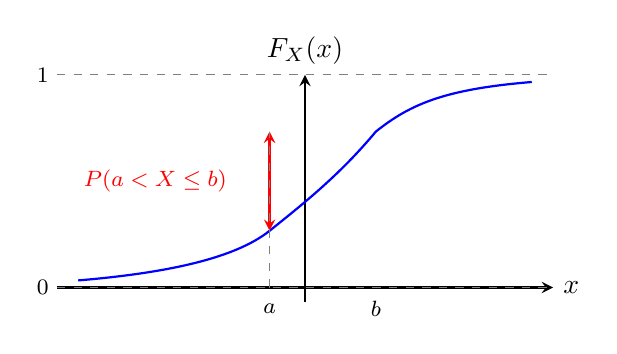
\begin{tikzpicture}[scale=0.9]

  \draw[->, thick, >=stealth] (-3.5,0) -- (3.5,0) node[right] {$x$};
  \draw[->, thick, >=stealth] (0,-0.2) -- (0,3) node[above] {$F_X(x)$};

  \draw[thick, blue] (-3.2,0.1) .. controls (-2,0.2) and (-1,0.4) .. (-0.5,0.8)
                                .. controls (0,1.2) and (0.5,1.6) .. (1,2.2)
                                .. controls (1.5,2.6) and (2,2.8) .. (3.2,2.9);

  \draw[gray, dashed] (-3.5,0) -- (3.5,0);
  \draw[gray, dashed] (-3.5,3) -- (3.5,3);
  \node[font=\footnotesize] at (-3.7,0) {$0$};
  \node[font=\footnotesize] at (-3.7,3) {$1$};

  \draw[<->, thick, red, >=stealth] (-0.5,0.8) -- (-0.5,2.2);
  \node[red, font=\footnotesize, xshift=-1cm] at (-1.0,1.5) {$\mathbb P(a<X\le b)$};
  \draw[gray, dashed] (-0.5,0) -- (-0.5,2.2);
  \node[font=\footnotesize] at (-0.5,-0.3) {$a$};
  \node[font=\footnotesize] at (1,-0.3) {$b$};
\end{tikzpicture}
\caption{累积分布函数的性质：单调不减、右连续、区间概率由端点差给出。}
\label{fig:cdf_properties}
\end{figure}

\begin{theorem}[CDF与分布的一一对应]\label{thm:cdf_uniqueness}
两个随机变量 $X$ 和 $Y$ 具有相同的分布当且仅当它们的累积分布函数相等：$F_X = F_Y$。
\end{theorem}

\begin{proof}
必要性：若 $X\stackrel{d}{=}Y$，则对一切 $x$ 有 $\mathbb P(X\le x)=\mathbb P(Y\le x)$，即 $F_X=F_Y$。充分性：设 $F_X = F_Y$。对任意 $a < b$，由性质 \ref{prop:cdf_properties}(iv) 得 $\mathbb{P}(a < X \le b) = \mathbb{P}(a < Y \le b)$。对任意半开区间 $(a, b]$，两随机变量的概率相等。由半开区间族生成的 $\sigma$-代数即 Borel $\sigma$-代数 $\mathcal{B}(\mathbb{R})$，故两随机变量在 $\mathcal{B}(\mathbb{R})$ 上诱导相同的概率测度，即同分布。
\end{proof}

\begin{definition}[分位数函数]\label{def:quantile}
设 $F_X$ 为随机变量 $X$ 的累积分布函数。$X$ 的\textbf{分位数函数}（广义反函数）定义为
\[
F_X^{-1}(p) = \inf\{x \in \mathbb{R} : F_X(x) \ge p\}, \qquad p \in (0, 1).
\]
特别地，$F_X^{-1}(1/2)$ 称为\textbf{中位数}，$F_X^{-1}(1/4)$ 和 $F_X^{-1}(3/4)$ 分别称为第一和第三四分位数。
\end{definition}

\begin{proposition}[分位数函数的基本性质]\label{prop:quantile_properties}
设 $F_X^{-1}$ 为随机变量 $X$ 的分位数函数。则
\begin{enumerate}[label=(\roman*)]
    \item \textbf{单调不减}：$p_1 \le p_2 \Rightarrow F_X^{-1}(p_1) \le F_X^{-1}(p_2)$。
    \item \textbf{左连续}：$F_X^{-1}$ 在 $(0,1)$ 上左连续。
    \item \textbf{与CDF的伴随关系}：$F_X^{-1}(p) \le x \iff p \le F_X(x)$。
\end{enumerate}
\end{proposition}

\begin{proof}
(i) 若 $p_1 \le p_2$，则 $\{x : F_X(x) \ge p_2\} \subseteq \{x : F_X(x) \ge p_1\}$，下确界单调。

(ii) 设 $p_n \uparrow p$。由 (i)，$F_X^{-1}(p_n)$ 递增且 $\le F_X^{-1}(p)$。设其极限为 $L \le F_X^{-1}(p)$。由 (iii) 待证的等价关系，$F_X^{-1}(p_n) \le x \iff p_n \le F_X(x)$。取 $x = L$，由右连续性得 $p \le F_X(L)$，故 $F_X^{-1}(p) \le L$，从而 $L = F_X^{-1}(p)$。

(iii) 若 $p \le F_X(x)$，则 $x \in \{y : F_X(y) \ge p\}$，故 $F_X^{-1}(p) \le x$。反之若 $F_X^{-1}(p) \le x$，由 $F_X$ 单调不减及 $F_X(F_X^{-1}(p)) \ge p$，得 $F_X(x) \ge p$。
\end{proof}

\subsection{离散分布与连续分布}

\begin{definition}[离散分布]\label{def:discrete_distribution}
设 $X$ 为取值于有限或可数集合 $\{x_0 < x_1 < \cdots\}$ 的随机变量。$X$ 的\textbf{概率质量函数}（PMF）为 $p_X(k) = \mathbb{P}(X = x_k)$，满足
\[
p_X(k) \ge 0, \quad \sum_{k} p_X(k) = 1.
\]
\end{definition}

\begin{proposition}[离散分布的概率质量函数与CDF]\label{prop:pmf_cdf_relation}
设 $X$ 为取值于 $\{x_0 < x_1 < \cdots\}$ 的离散随机变量，$p_k = \mathbb{P}(X = x_k)$。则
\[
F_X(x) = \sum_{k : x_k \le x} p_k.
\]
\end{proposition}

\begin{proof}
$\{X \le x\} = \bigcup_{k: x_k \le x} \{X = x_k\}$ 为可数不相交并，由可数可加性即得。
\end{proof}

\begin{proposition}[任何有限离散分布都是循环群上的分布]
\label{prop:discrete_cyclic}
设 $X$ 是一个离散随机变量，取值于有限集合
\[
\{x_0, x_1, \dots, x_{N-1}\}.
\]
通过双射 $x_k \mapsto k \in C_N$，
$X$ 等价于 $C_N$ 上的概率分布 $(p_0, p_1, \dots, p_{N-1})$，
其中 $p_k = \mathbb{P}(X = x_k)$。
\end{proposition}
\begin{proof}
构造双射 $\varphi(x_k) = k$。定义 $p(k) = \mathbb{P}(X = x_k)$。总质量 $\sum_{k=0}^{N-1} p(k) = 1$。这是有限集合上概率分布的标准重参数化，不构成新的数学内容。
\end{proof}

\begin{proposition}[循环群上的平移不变分布]\label{prop:cyclic_uniform}
$C_N$ 上唯一的平移不变概率分布是均匀分布 $p(k) = 1/N$。对任意 $a \in C_N$，$p(k+a) = p(k)$ 迫使 $p$ 为常数。
\end{proposition}

\begin{proof}
平移不变要求 $p(k+a) = p(k)$ 对所有 $k, a \in C_N$。取 $a=1$ 得 $p(k+1) = p(k)$ 对所有 $k$，故 $p$ 为常函数。由归一化得 $p(k) = 1/N$。这是 $C_N$ 上的 Haar 测度。
\end{proof}

\begin{definition}[连续分布]\label{def:continuous_distribution}
随机变量 $X$ 称为\textbf{连续型}的，若存在\textbf{概率密度函数}（PDF）$f_X(x)$ 使得 $\mathbb{P}(X \in B) = \int_B f_X(x) dx$ 对所有 $B \in \mathcal{B}(\mathbb{R})$ 成立。密度与累积分布函数的关系为 $F_X(x) = \int_{-\infty}^{x} f_X(t) dt$，且在 $f_X$ 连续处 $F_X' = f_X$。
\end{definition}

\section{随机变量与常见分布}\label{sec:common_distributions}

\subsection{离散型随机变量}

\begin{definition}[伯努利分布与二项分布]\label{def:bernoulli_binomial}
伯努利随机变量 $X \sim \operatorname{Bernoulli}(p)$ 是 $C_2$ 上的分布：$\mathbb{P}(X=1) = p$，$\mathbb{P}(X=0) = 1-p$。

$n$ 次独立伯努利试验的成功次数 $X \sim \operatorname{Binomial}(n, p)$ 是 $C_{n+1} = \{0, 1, \dots, n\}$ 上的分布：
\[
\mathbb{P}(X = k) = \binom{n}{k} p^k (1-p)^{n-k}, \quad k = 0, 1, \dots, n.
\]
期望 $\mathbb{E}[X] = np$，方差 $\operatorname{Var}(X) = np(1-p)$。
\end{definition}

\begin{definition}[泊松分布]\label{def:poisson_distribution}
泊松分布 $X \sim \operatorname{Poisson}(\lambda)$ 是 $\mathbb{N}$ 上的分布：
\[
\mathbb{P}(X = k) = \frac{\lambda^k e^{-\lambda}}{k!}, \quad k = 0, 1, 2, \dots.
\]
期望和方差均为 $\lambda$。泊松分布是二项分布在 $n \to \infty$、$np \to \lambda$ 下的极限分布。
\end{definition}

\begin{definition}[几何分布与负二项分布]\label{def:geometric_negbinomial}
几何分布 $X \sim \operatorname{Geometric}(p)$ 是首次成功所需的试验次数：
\[
\mathbb{P}(X = k) = (1-p)^{k-1} p, \quad k = 1, 2, \dots.
\]
期望 $\mathbb{E}[X] = 1/p$，方差 $\operatorname{Var}(X) = (1-p)/p^2$。几何分布具有无记忆性。

负二项分布 $X \sim \operatorname{NegBinomial}(r, p)$ 是第 $r$ 次成功所需的试验次数：
\[
\mathbb{P}(X = k) = \binom{k-1}{r-1} p^r (1-p)^{k-r}, \quad k = r, r+1, \dots.
\]
期望 $\mathbb{E}[X] = r/p$，方差 $\operatorname{Var}(X) = r(1-p)/p^2$。
\end{definition}

\begin{figure}[htbp]
\centering
\begin{tikzpicture}[scale=0.9]

  \draw[->, thick, >=stealth] (-0.5,0) -- (8,0) node[right] {$k$};
  \draw[->, thick, >=stealth] (0,-0.2) -- (0,2.5) node[above] {$\mathbb P(X=k)$};

  \foreach \k/\h in {0/0.028,1/0.121,2/0.233,3/0.267,4/0.200,5/0.103,6/0.037,7/0.009} {
    \fill[blue!60] (\k*0.9,0) rectangle (\k*0.9+0.6,\h*8);
    \node[font=\scriptsize] at (\k*0.9+0.3,-0.15) {\k};
  }
  \node[blue, yshift=0.5cm] at (4,2.2) {二项 $B(10,0.3)$};
\end{tikzpicture}
\caption{二项分布 $B(10,0.3)$ 的概率质量函数。}
\label{fig:binomial_pmf}
\end{figure}

\subsection{连续型随机变量}

\begin{definition}[均匀分布]\label{def:uniform_distribution}
$X \sim \operatorname{Uniform}(a, b)$ 的密度为 $f_X(x) = \frac{1}{b-a}$（$a \le x \le b$）。$S^1$ 上的均匀分布是圆群上的 Haar 测度，具有完全的旋转对称性。
\end{definition}

\begin{proposition}[$S^1$ 上均匀分布的旋转不变性]\label{prop:S1_uniform_rotation}
设 $X$ 在 $S^1 = \mathbb{R}/(2\pi\mathbb{Z})$ 上均匀分布（密度 $f_X(\theta) = 1/(2\pi)$）。则对任意 $\phi \in S^1$，$X + \phi$（模 $2\pi$）仍均匀分布。$S^1$ 上均匀分布是唯一具有旋转不变性的概率分布。
\end{proposition}

\begin{proof}
密度 $f_{X+\phi}(\theta) = f_X(\theta - \phi) = 1/(2\pi)$，与 $\phi$ 无关。反之若 $f$ 旋转不变，则 $f(\theta - \phi) = f(\theta)$ 对所有 $\phi$ 成立，$f$ 为常数，由归一化得 $f = 1/(2\pi)$。
\end{proof}

\begin{definition}[正态分布]\label{def:normal_distribution}
$X \sim \mathcal{N}(\mu, \sigma^2)$ 的密度为
\[
f_X(x) = \frac{1}{\sqrt{2\pi}\sigma} e^{-(x-\mu)^2/(2\sigma^2)}.
\]
$\mu$ 是期望，$\sigma^2$ 是方差。正态分布是中心极限定理的极限分布。
\end{definition}

\begin{definition}[指数分布]\label{def:exponential_distribution}
$X \sim \operatorname{Exponential}(\lambda)$ 的密度为 $f_X(x) = \lambda e^{-\lambda x}$（$x \ge 0$）。具有无记忆性：$\mathbb{P}(X > s + t \mid X > s) = \mathbb{P}(X > t)$。期望 $1/\lambda$，方差 $1/\lambda^2$。
\end{definition}

\begin{definition}[伽马分布]\label{def:gamma_distribution}
$X \sim \operatorname{Gamma}(\alpha, \beta)$ 的密度为
\[
f_X(x) = \frac{\beta^\alpha}{\Gamma(\alpha)} x^{\alpha-1} e^{-\beta x}, \quad x > 0,
\]
其中 $\alpha > 0$ 是形状参数，$\beta > 0$ 是速率参数，$\Gamma(\alpha) = \int_0^\infty t^{\alpha-1} e^{-t} dt$ 是伽马函数。期望 $\alpha/\beta$，方差 $\alpha/\beta^2$。指数分布是 $\alpha = 1$ 的特例。
\end{definition}

\begin{definition}[贝塔分布]\label{def:beta_distribution}
$X \sim \operatorname{Beta}(\alpha, \beta)$ 的密度为
\[
f_X(x) = \frac{x^{\alpha-1} (1-x)^{\beta-1}}{B(\alpha, \beta)}, \quad x \in (0, 1),
\]
其中 $B(\alpha, \beta) = \Gamma(\alpha)\Gamma(\beta)/\Gamma(\alpha+\beta)$ 是贝塔函数。期望 $\alpha/(\alpha+\beta)$，方差 $\alpha\beta/[(\alpha+\beta)^2(\alpha+\beta+1)]$。均匀分布 $\operatorname{Uniform}(0,1)$ 是 $\alpha = \beta = 1$ 的特例。
\end{definition}

\begin{definition}[卡方分布、$t$分布与$F$分布]\label{def:chi2_t_f}
设 $Z_1, \dots, Z_n$ 为独立标准正态随机变量。
\begin{enumerate}[label=(\roman*)]
    \item \textbf{卡方分布}：$X = \sum_{i=1}^n Z_i^2 \sim \chi^2(n)$，是 $\operatorname{Gamma}(n/2, 1/2)$ 的特例，期望 $n$，方差 $2n$。
    \item \textbf{$t$分布}：若 $Z \sim \mathcal{N}(0,1)$ 与 $V \sim \chi^2(n)$ 独立，则 $T = Z/\sqrt{V/n} \sim t(n)$，期望 $0$（$n > 1$），方差 $n/(n-2)$（$n > 2$）。
    \item \textbf{$F$分布}：若 $U \sim \chi^2(m)$ 与 $V \sim \chi^2(n)$ 独立，则 $F = (U/m)/(V/n) \sim F(m, n)$。
\end{enumerate}
\end{definition}

\begin{figure}[htbp]
\centering
\begin{tikzpicture}[scale=0.9]

  \draw[->, thick, >=stealth] (-4,0) -- (4,0) node[right] {$x$};
  \draw[->, thick, >=stealth] (0,-0.2) -- (0,2.5) node[above] {密度};

  \draw[thick, blue, domain=-3.5:3.5, samples=100] plot (\x, {2*exp(-\x*\x/2)});
  \node[blue, font=\footnotesize] at (2.0,1.8) {$\mathcal N(0,1)$};

  \draw[thick, red] (-2,0) -- (-2,0.6) -- (2,0.6) -- (2,0);
  \node[red, font=\footnotesize, yshift=0.5cm] at (2.8,0.6) {$\mathrm{Unif}(-2,2)$};

  \draw[thick, green!60!black, domain=0:3.5, samples=50] plot (\x, {2*exp(-2*\x)});
  \node[green!60!black, font=\footnotesize, xshift=0.5cm] at (2.5,0.4) {$\mathrm{Exp}(2)$};
\end{tikzpicture}
\caption{三种连续分布的密度函数对比：正态、均匀、指数。}
\label{fig:continuous_pdf}
\end{figure}

\subsection{常见分布的关系}

\begin{proposition}[常见分布之间的极限与特例关系]\label{prop:distribution_relations}
\begin{enumerate}[label=(\roman*)]
    \item \textbf{二项到泊松}：$\operatorname{Binomial}(n, \lambda/n) \xrightarrow{d} \operatorname{Poisson}(\lambda)$（$n \to \infty$）。
    \item \textbf{二项到正态}：$\frac{X - np}{\sqrt{np(1-p)}} \xrightarrow{d} \mathcal{N}(0,1)$（$n \to \infty$，De Moivre–Laplace 定理）。
    \item \textbf{伽马到正态}：$\frac{X - \alpha/\beta}{\sqrt{\alpha/\beta^2}} \xrightarrow{d} \mathcal{N}(0,1)$（$\alpha \to \infty$）。
    \item \textbf{$t$分布到正态}：$t(n) \xrightarrow{d} \mathcal{N}(0,1)$（$n \to \infty$）。
    \item \textbf{贝塔到正态}：$\frac{X - \mu}{\sigma} \xrightarrow{d} \mathcal{N}(0,1)$（$\alpha, \beta \to \infty$，其中 $\mu = \alpha/(\alpha+\beta)$，$\sigma^2 = \alpha\beta/[(\alpha+\beta)^2(\alpha+\beta+1)]$）。
\end{enumerate}
\end{proposition}

\begin{proof}
(i) 由泊松极限定理（概率生成函数或特征函数的极限给出）。(ii) 由中心极限定理（定理 \ref{thm:central_limit_theorem}）应用于 $n$ 个独立伯努利随机变量之和。(iii)(iv)(v) 由特征函数的大参数渐近展开（鞍点法）直接验证。五条均为经典结果。
\end{proof}

\begin{figure}[htbp]
\centering
\begin{tikzpicture}[
  font=\small,
  box/.style={draw, rounded corners, fill=blue!8, minimum width=2.2cm, minimum height=0.7cm, align=center, font=\footnotesize},
  arr/.style={->, thick, >=stealth}
]
  \node[box] (bern) {Bernoulli};
  \node[box, right=1.0cm of bern] (bin) {Binomial};
  \node[box, right=1.0cm of bin] (pois) {Poisson};
  \node[box, below=0.8cm of bin] (norm) {Normal};
  \node[box, below=0.8cm of bern] (exp) {Exponential};
  \node[box, right=1.0cm of exp] (gamma) {Gamma};
  \node[box, right=1.0cm of gamma] (chi2) {$\chi^2$};
  \node[box, below=0.8cm of gamma] (beta) {Beta};
  \node[box, right=1.0cm of norm] (t) {$t$};
  \node[box, right=1.0cm of t] (F) {$F$};
  \draw[arr] (bern) -- (bin);
  \draw[arr] (bin) -- node[above, font=\scriptsize]{$n\to\infty$} (pois);
  \draw[arr] (bin) -- node[right, font=\scriptsize]{CLT} (norm);
  \draw[arr] (exp) -- (gamma);
  \draw[arr] (gamma) -- (chi2);
  \draw[arr] (gamma) -- (beta);
  \draw[arr] (norm) -- (t);
  \draw[arr] (chi2) -- (F);
\end{tikzpicture}
\caption{常见分布之间的极限与特例关系图。}
\label{fig:distribution_relations}
\end{figure}

\section{特征函数}\label{sec:characteristic_function}

\begin{definition}[特征函数]\label{def:characteristic_function}
随机变量 $X$ 的\textbf{特征函数}定义为
\[
\phi_X(t) = \mathbb{E}[e^{itX}] =
\begin{cases}
\sum_k e^{itk} p_X(k) & \text{（离散型）} \\
\int_{-\infty}^{\infty} e^{itx} f_X(x) dx & \text{（连续型）}
\end{cases}, \quad t \in \mathbb{R}.
\]
\end{definition}

\begin{theorem}[特征函数是分布的傅里叶变换]\label{thm:characteristic_fourier}
特征函数 $\phi_X(t)$ 正是分布测度 $\mu_X$ 关于特征 $x \mapsto e^{itx}$ 的傅里叶变换 $\widehat{\mu}_X(t)$：离散型 $\phi_X(t) = \sum_k e^{itk} p_X(k)$，连续型 $\phi_X(t) = \int_{-\infty}^{\infty} e^{itx} f_X(x)\,dx$。写成极坐标 $\phi_X(t) = |\phi_X(t)| e^{i\arg\phi_X(t)}$：模 $|\phi_X(t)|$ 度量频率 $t$ 处的相干叠加强度，辐角 $\arg\phi_X(t)$ 度量复相位偏移。
\end{theorem}

\begin{proof}
由定义 \ref{def:characteristic_function}，$\phi_X(t) = \mathbb{E}[e^{itX}] = \int e^{itx} d\mu_X(x)$，这正是分布测度 $\mu_X$ 的傅里叶变换。极坐标分解 $|\phi_X(t)| e^{i\arg\phi_X(t)}$ 给出模与辐角两个分量。
\end{proof}

\begin{proposition}[特征函数的基本性质]\label{prop:characteristic_function_properties}
\begin{enumerate}[label=(\roman*)]
    \item $\phi_X(0) = 1$，$|\phi_X(t)| \le 1$。
    \item 若 $X$ 和 $Y$ 独立，则 $\phi_{X+Y}(t) = \phi_X(t) \phi_Y(t)$。
    \item $\mathbb{E}[X^n] = i^{-n} \phi_X^{(n)}(0)$——矩是特征函数在 $t=0$ 处的导数。
    \item 特征函数唯一确定分布。
    \item $\phi_{aX+b}(t) = e^{ibt} \phi_X(at)$（线性变换）。
\end{enumerate}
\end{proposition}

\begin{proof}
(i) $\phi_X(0) = \mathbb{E}[e^{0}] = 1$；又 $|\phi_X(t)| \le \mathbb{E}|e^{itX}| = 1$。
(ii) 由独立性，$\phi_{X+Y}(t) = \mathbb{E}[e^{it(X+Y)}] = \mathbb{E}[e^{itX}]\,\mathbb{E}[e^{itY}] = \phi_X(t)\phi_Y(t)$。
(iii) 在期望号下求导：$\phi_X^{(n)}(t) = i^n \mathbb{E}[X^n e^{itX}]$，取 $t = 0$ 得 $\phi_X^{(n)}(0) = i^n \mathbb{E}[X^n]$。
(iv) 由 Lévy 反演公式，分布函数 $F_X$ 可由 $\phi_X$ 唯一恢复。
(v) $\phi_{aX+b}(t) = \mathbb{E}[e^{it(aX+b)}] = e^{ibt} \mathbb{E}[e^{i(at)X}] = e^{ibt} \phi_X(at)$。
\end{proof}

\begin{remark}[特征函数与分布的三类信息]\label{prop:characteristic_grammar}
特征函数 $\phi_X$ 包含分布的三类信息：
\begin{enumerate}[label=(\roman*)]
    \item \textbf{矩信息}：$\phi_X^{(n)}(0) = i^n \mathbb{E}[X^n]$——$\phi_X$ 在 $t = 0$ 处的各阶导数给出分布的各阶矩。期望 $\mathbb{E}[X] = -i\phi_X'(0)$，方差 $\operatorname{Var}(X) = -\phi_X''(0) + \phi_X'(0)^2$。
    \item \textbf{模信息}：$|\phi_X(t)|$ 度量频率 $t$ 处的相干叠加强度。
    \item \textbf{衰减信息}：当 $|t| \to \infty$ 时 $|\phi_X(t)|$ 的衰减速率反映分布尾部的特征。
\end{enumerate}
\end{remark}

\begin{figure}[htbp]
\centering
\begin{tikzpicture}[scale=0.9]

  \draw[->, thick, >=stealth] (-3.5,0) -- (3.5,0) node[right] {$t$};
  \draw[->, thick, >=stealth] (0,-0.2) -- (0,2.5) node[above] {$|\phi_X(t)|$};

  \draw[thick, blue, domain=-3.5:3.5, samples=100] plot (\x, {2*exp(-\x*\x/2)});
  \node[blue, font=\footnotesize] at (2.5,1.8) {正态：$e^{-\sigma^2t^2/2}$};

  \draw[thick, red, domain=-3.5:3.5, samples=100] plot (\x, {2*exp(-2*(1-cos(\x r)))});
  \node[red, font=\footnotesize, xshift=1cm] at (2.5,0.6) {泊松：$e^{\lambda(\cos t-1)}$};

  \draw[thick, green!60!black, domain=-3.5:3.5, samples=100] plot (\x, {abs(sin(\x r)/(\x r))*2});
  \node[green!60!black, font=\footnotesize] at (2.8,1.2) {均匀：$|\sin t/t|$};
\end{tikzpicture}
\caption{三种分布的特征函数模 $|\phi_X(t)|$：正态（高斯衰减）、泊松（周期振荡衰减）、均匀（sinc 衰减）。}
\label{fig:characteristic_functions}
\end{figure}

\begin{lemma}[特征函数的正定性]\label{ch14_characteristic_pd}
设 $\phi_X$ 为随机变量 $X$ 的特征函数。则对任意 $n \in \mathbb{N}^+$、任意 $t_1, \dots, t_n \in \mathbb{R}$ 与任意复数 $z_1, \dots, z_n$，
\[
\sum_{j,k=1}^{n} z_j \overline{z_k}\, \phi_X(t_j - t_k) \ge 0,
\]
即矩阵 $\bigl( \phi_X(t_j - t_k) \bigr)_{j,k=1}^{n}$ 半正定。
\end{lemma}

\begin{proof}
由定义 \ref{def:characteristic_function} 与期望的线性性：
\[
\sum_{j,k} z_j \overline{z_k}\, \phi_X(t_j - t_k)
= \mathbb{E}\Big[ \sum_{j,k} z_j \overline{z_k}\, e^{i(t_j - t_k) X} \Big]
= \mathbb{E}\Big[ \Big| \sum_{j} z_j e^{it_j X} \Big|^2 \Big] \ge 0.
\]
\end{proof}

\begin{example}[泊松分布特征函数的具体计算]\label{ch14_poisson_char_example}
设 $X \sim \operatorname{Poisson}(\lambda)$。则
\[
\phi_X(t) = \sum_{k=0}^{\infty} e^{itk}\, \frac{\lambda^k e^{-\lambda}}{k!}
= e^{-\lambda} \sum_{k=0}^{\infty} \frac{(\lambda e^{it})^k}{k!}
= e^{\lambda (e^{it} - 1)}.
\]
取 $\lambda = 2$、$t = \pi/2$：$\phi_X(\pi/2) = e^{2(i-1)} = e^{-2} e^{2i} \approx 0.1353 \cdot (-0.4161 + 0.9093 i) \approx -0.0563 + 0.1230 i$。模 $|\phi_X(\pi/2)| = e^{-2} \approx 0.1353$。
\end{example}

\begin{example}[二项分布特征函数的具体计算]\label{ch14_binomial_char_example}
设 $X \sim \operatorname{Binomial}(n, p)$。则
\[
\phi_X(t) = (p e^{it} + 1 - p)^n.
\]
取 $n = 3$、$p = 1/2$：$\phi_X(t) = \tfrac18 (e^{it} + 1)^3$。代入 $t = \pi$：$\phi_X(\pi) = (-\tfrac12 + \tfrac12)^3 = 0$，与直接求和一致。
\end{example}

\begin{example}[正态分布的特征函数]\label{ex:normal_characteristic}
若 $X \sim \mathcal{N}(\mu, \sigma^2)$，则 $\phi_X(t) = e^{i\mu t - \sigma^2 t^2/2}$。模 $|\phi_X(t)| = e^{-\sigma^2 t^2/2}$ 是高斯核。辐角 $\arg \phi_X(t) = \mu t$ 是线性相位。
\end{example}

\begin{example}[伽马分布的特征函数]\label{ex:gamma_characteristic}
若 $X \sim \operatorname{Gamma}(\alpha, \beta)$，则 $\phi_X(t) = (1 - it/\beta)^{-\alpha}$（$t \in \mathbb{R}$）。指数分布（$\alpha = 1$）的特征函数为 $\phi_X(t) = (1 - it/\lambda)^{-1}$。
\end{example}

\begin{remark}[特征函数在整数频率处的取值]\label{ch14_periodic_series_interface}
设 $X$ 为 $S^1$ 上的随机变量，质量密度为 $f_X$。则 $f_X$ 的傅里叶系数为
\[
c_n = \frac{1}{2\pi} \int_0^{2\pi} f_X(\theta)\, e^{-in\theta}\, d\theta = \frac{1}{2\pi}\mathbb{E}[e^{-inX}] = \frac{\phi_X(-n)}{2\pi}.
\]
即 $c_n = \phi_X(-n)/(2\pi)$：特征函数在整数频率处的取值是密度函数的傅里叶系数的 $2\pi$ 倍。这一对应是周期数学与概率论的核心接口：\textbf{概率分布的特征函数在整数点的取值恰为其密度傅里叶系数的 $2\pi$ 倍}。
\end{remark}

\begin{proposition}[$S^1$ 上分布的特征函数与傅里叶系数]\label{prop:S1_char_fourier}
设 $X$ 为 $S^1$ 上的随机变量，密度 $f_X \in L^1(S^1)$。则：
\begin{enumerate}[label=(\roman*)]
    \item 归一化特征函数的共轭 $\phi_X(-n)/(2\pi)$ 是密度的傅里叶系数 $c_n$，即 $\phi_X(-n) = 2\pi c_n$（等价地 $\phi_X(n) = 2\pi c_{-n}$，$n \in \mathbb{Z}$）；
    \item 密度可由特征函数重构：$f_X(\theta) = \frac{1}{2\pi}\sum_{n \in \mathbb{Z}} \phi_X(n) e^{in\theta}$（在 $L^2$ 意义下）；
    \item 帕塞瓦尔恒等式：$\sum_{n \in \mathbb{Z}} |\phi_X(n)|^2 = 2\pi \int_{S^1} |f_X(\theta)|^2 d\theta$。
\end{enumerate}
\end{proposition}

\begin{proof}
(i) 直接由定义 \ref{def:characteristic_function} 与傅里叶系数定义。(ii) 由傅里叶逆变换公式。(iii) 由 $L^2(S^1)$ 上的帕塞瓦尔恒等式。
\end{proof}

\section{贝叶斯推断}\label{sec:bayesian_inference}

\subsection{贝叶斯推断的基本框架}
\label{subsec:bayes_framework}

\begin{definition}[贝叶斯推断的基本框架]\label{def:bayesian_inference}
\textbf{贝叶斯推断}是将未知参数 $\theta$ 视为随机变量，通过观测数据 $\mathbf{D}$ 更新对 $\theta$ 认知的方法。三个基本要素为：
\begin{enumerate}[label=(\roman*)]
    \item \textbf{先验分布} $\pi(\theta)$：观测前的分布。
    \item \textbf{似然函数} $p(\mathbf{D} \mid \theta)$：给定参数 $\theta$ 时观测数据的概率。
    \item \textbf{后验分布} $p(\theta \mid \mathbf{D})$：观测后的分布，由贝叶斯定理给出：
    \[
    p(\theta \mid \mathbf{D}) = \frac{p(\mathbf{D} \mid \theta) \pi(\theta)}{p(\mathbf{D})}.
    \]
\end{enumerate}
\end{definition}

\begin{definition}[共轭先验]\label{def:conjugate_prior}
设 $\mathcal{F} = \{p(\mathbf{D} \mid \theta)\}$ 为似然函数族。先验分布族 $\mathcal{G}$ 称为 $\mathcal{F}$ 的\textbf{共轭先验}族，若对任意 $\pi \in \mathcal{G}$ 和任意数据 $\mathbf{D}$，后验 $p(\theta \mid \mathbf{D})$ 仍属于 $\mathcal{G}$。共轭先验是分布族在贝叶斯更新下封闭的族。
\end{definition}

\begin{figure}[htbp]
\centering
\begin{tikzpicture}[font=\small, arr/.style={->, thick, >=stealth}]
  \node[draw, rounded corners, fill=blue!8, minimum width=2.6cm, minimum height=0.8cm] (prior) {先验 $\pi(\theta)$};
  \node[draw, rounded corners, fill=orange!12, minimum width=2.6cm, minimum height=0.8cm, right=1.0cm of prior] (like) {似然 $p(\mathbf D|\theta)$};
  \node[draw, rounded corners, fill=green!12, minimum width=2.6cm, minimum height=0.8cm, right=1.0cm of like] (post) {后验 $p(\theta|\mathbf D)$};
  \draw[arr] (prior) -- (like);
  \draw[arr] (like) -- (post);
  \node[font=\footnotesize] at (3,-1.0) {贝叶斯更新：先验 $\times$ 似然 $\propto$ 后验};
\end{tikzpicture}
\caption{贝叶斯推断的三要素：先验、似然、后验。}
\label{fig:bayes_framework}
\end{figure}

\begin{example}[Beta-二项共轭模型]\label{ex:beta_binomial}
设似然为 $X \mid \theta \sim \operatorname{Binomial}(n, \theta)$，先验为 $\theta \sim \operatorname{Beta}(\alpha, \beta)$。则后验为 $\theta \mid X = x \sim \operatorname{Beta}(\alpha + x, \beta + n - x)$。先验参数 $(\alpha, \beta)$ 被更新为 $(\alpha + x, \beta + n - x)$——先验的“伪观测计数”与实际观测计数相加。
\end{example}

\begin{example}[Beta-二项共轭更新的数值算例]\label{ch14_beta_binomial_numeric}
设似然为 $X \mid \theta \sim \operatorname{Binomial}(10, \theta)$，先验为 $\theta \sim \operatorname{Beta}(2, 2)$，观测到 $x = 7$ 次成功。后验为 $\theta \mid X = 7 \sim \operatorname{Beta}(9, 5)$。
\begin{itemize}
    \item 先验均值：$\mathbb{E}[\theta] = 0.5$；后验均值：$\mathbb{E}[\theta \mid \mathbf{D}] = 9/14 \approx 0.6429$；
    \item 后验方差：$\operatorname{Var}(\theta \mid \mathbf{D}) = 3/196 \approx 0.01531$；
    \item 后验众数：$2/3 \approx 0.6667$。
\end{itemize}
先验的伪计数 $(1, 1)$ 与真实观测 $(7, 3)$ 相加得后验伪计数 $(8, 6)$。
\end{example}

\begin{example}[正态-正态共轭模型]\label{ex:normal_normal}
设似然为 $X_1, \dots, X_n \mid \mu \sim \mathcal{N}(\mu, \sigma^2)$（$\sigma^2$ 已知），先验为 $\mu \sim \mathcal{N}(\mu_0, \tau^2)$。则后验为
\[
\mu \mid \mathbf{D} \sim \mathcal{N}\left( \frac{\frac{1}{\tau^2}\mu_0 + \frac{n}{\sigma^2}\bar{x}}{\frac{1}{\tau^2} + \frac{n}{\sigma^2}}, \; \frac{1}{\frac{1}{\tau^2} + \frac{n}{\sigma^2}} \right).
\]
\end{example}

\begin{example}[伽马–泊松共轭模型]
\label{ex:gamma_poisson}
设似然为
\[
X \mid \lambda \sim \operatorname{Poisson}(\lambda),
\]
先验为 $\lambda \sim \operatorname{Gamma}(\alpha, \beta)$。
则后验为
\[
\lambda \mid X = x \sim \operatorname{Gamma}(\alpha + x, \beta + 1).
\]
先验的形状参数增加观测次数，速率参数增加 $1$。
\end{example}

\begin{definition}[边际似然]\label{def:marginal_likelihood}
\textbf{边际似然}为 $p(\mathbf{D}) = \int_{\Theta} p(\mathbf{D} \mid \theta) \pi(\theta) d\theta$。边际似然是先验分布与似然权重的整体积分。
\end{definition}

\subsection{序贯贝叶斯更新与后验收敛}

\begin{definition}[序贯贝叶斯更新]\label{def:sequential_bayesian}
设初始先验为 $\pi_0(\theta)$，观测数据依次为 $\mathbf{D}_1, \mathbf{D}_2, \dots$。序贯贝叶斯更新为
\[
p_k(\theta) \propto p(\mathbf{D}_k \mid \theta) p_{k-1}(\theta), \quad k = 1, 2, \dots.
\]
\end{definition}

\begin{theorem}[Bernstein-von Mises 定理]\label{thm:bernstein_von_mises}
设 $\mathbf{D} = (X_1, \dots, X_n)$ 为独立同分布样本，$\theta_0$ 为真实参数，先验 $\pi(\theta)$ 在 $\theta_0$ 处连续且为正。则在适当正则条件下，
\[
\sqrt{n}(\theta - \hat{\theta}_n) \mid \mathbf{D} \xrightarrow{d} \mathcal{N}(0, \mathcal{I}(\theta_0)^{-1}).
\]
后验分布在大样本下收敛于正态分布。
\end{theorem}

\begin{proof}[证明思路]
先验在 $\theta_0$ 附近近似为常数，后验与似然成正比。对数似然在极大似然估计处泰勒展开至二阶，得后验密度渐近正比于 $\exp(-\tfrac12 \mathcal{I}(\theta_0) u^2)$，即 $\mathcal{N}(0, \mathcal{I}(\theta_0)^{-1})$。严格论证见 van der Vaart, \emph{Asymptotic Statistics}（1998）第 10 章。
\end{proof}

\begin{proposition}[贝叶斯周期参数估计]\label{prop:bayesian_periodic_diagnosis}
对于具有周期结构的随机过程，贝叶斯推断可用于估计周期参数。后验 $p(T \mid \mathbf{D})$ 在真实周期处出现尖峰，最大后验估计 $\hat{T}_{\text{MAP}}$ 给出周期的最优估计。后验宽度度量估计不确定性——样本越多，后验越窄。
\end{proposition}

\begin{proof}
由 Bernstein-von Mises 定理（定理 \ref{thm:bernstein_von_mises}），
后验在大样本下近似于
\[
\mathcal{N}\!\bigl(T_0, [n\mathcal{I}(T_0)]^{-1}\bigr),
\]
故最大后验估计依概率收敛于 $T_0$，
后验宽度为 $O(n^{-1/2})$。
\end{proof}

\section{随机变量的数字特征}\label{sec:numerical_characteristics}

\begin{definition}[数学期望]\label{def:mathematical_expectation}
随机变量 $X$ 的\textbf{数学期望}为
\[
\mathbb{E}[X] =
\begin{cases}
\sum_k k p_X(k) & \text{（离散型）} \\
\int_{-\infty}^{\infty} x f_X(x) dx & \text{（连续型）}
\end{cases}.
\]
\end{definition}

\begin{property}[期望的基本性质]\label{prop:expectation_properties}
\begin{enumerate}[label=(\roman*)]
    \item \textbf{线性性}：$\mathbb{E}[aX + bY] = a\mathbb{E}[X] + b\mathbb{E}[Y]$。
    \item \textbf{独立可乘性}：若 $X, Y$ 独立，则 $\mathbb{E}[XY] = \mathbb{E}[X]\mathbb{E}[Y]$。
    \item \textbf{单调性}：若 $X \le Y$ 几乎处处，则 $\mathbb{E}[X] \le \mathbb{E}[Y]$。
\end{enumerate}
\end{property}

\begin{proof}
(i) 由积分的线性性。

(ii) 由独立性，联合分布可分解，
\[
\mathbb{E}[XY]
= \int xy \, dF_X(x)\,dF_Y(y)
= \mathbb{E}[X]\,\mathbb{E}[Y].
\]

(iii) 由 $Y - X \ge 0$ 几乎处处成立，
得 $\mathbb{E}[Y - X] \ge 0$。
\end{proof}

\begin{definition}[方差与标准差]\label{def:variance_std}
\[
\operatorname{Var}(X) = \mathbb{E}[(X - \mathbb{E}[X])^2] = \mathbb{E}[X^2] - (\mathbb{E}[X])^2.
\]
标准差 $\sigma_X = \sqrt{\operatorname{Var}(X)}$。
\end{definition}

\begin{property}[方差的基本性质]\label{prop:variance_properties}
\begin{enumerate}[label=(\roman*)]
    \item \textbf{平移不变性}：$\operatorname{Var}(X + b) = \operatorname{Var}(X)$。
    \item \textbf{缩放协变性}：$\operatorname{Var}(aX) = a^2 \operatorname{Var}(X)$。
    \item \textbf{独立可加性}：若 $X, Y$ 独立，则 $\operatorname{Var}(X + Y) = \operatorname{Var}(X) + \operatorname{Var}(Y)$。
\end{enumerate}
\end{property}

\begin{proof}
(i) $\operatorname{Var}(X + b) = \mathbb{E}[(X + b - \mathbb{E}[X] - b)^2] = \operatorname{Var}(X)$。(ii) $\operatorname{Var}(aX) = \mathbb{E}[a^2(X - \mathbb{E}[X])^2] = a^2 \operatorname{Var}(X)$。(iii) 由独立性，$\operatorname{Var}(X + Y) = \mathbb{E}[(X - \mathbb{E}[X])^2] + \mathbb{E}[(Y - \mathbb{E}[Y])^2] + 2\mathbb{E}[(X - \mathbb{E}[X])(Y - \mathbb{E}[Y])] = \operatorname{Var}(X) + \operatorname{Var}(Y)$。
\end{proof}

\begin{definition}[协方差与相关系数]\label{def:covariance}
随机变量 $X, Y$ 的\textbf{协方差}为 $\operatorname{Cov}(X, Y) = \mathbb{E}[(X - \mathbb{E}[X])(Y - \mathbb{E}[Y])]$。\textbf{相关系数}为 $\rho_{XY} = \operatorname{Cov}(X, Y)/(\sigma_X \sigma_Y)$，取值于 $[-1, 1]$。
\end{definition}

\begin{definition}[矩、偏度与峰度]\label{def:moments}
$k$ 阶原点矩 $\mu_k' = \mathbb{E}[X^k]$，$k$ 阶中心矩 $\mu_k = \mathbb{E}[(X - \mu)^k]$。\textbf{偏度}为 $\gamma_1 = \mu_3/\sigma^3$，\textbf{峰度}为 $\gamma_2 = \mu_4/\sigma^4 - 3$。
\end{definition}

\begin{definition}[熵]\label{def:entropy}
离散随机变量 $X$ 的\textbf{熵}为 $H(X) = -\sum_x p(x) \log p(x)$。连续随机变量 $X$ 的\textbf{微分熵}为 $h(X) = -\int f(x) \log f(x) dx$。熵度量了分布的均匀性。
\end{definition}

\begin{proposition}[均匀分布的最大熵]\label{prop:uniform_max_entropy}
在 $C_N$ 上，熵最大的是均匀分布 $p(k) = 1/N$，最大熵为 $H_{\max} = \log N$。
\end{proposition}

\begin{proof}
由对数不等式 $\log x \ge 1 - \frac{1}{x}$（$x > 0$），取 $x = N p_k$：
\[
\sum_{k} p_k \log(N p_k) \ge \sum_{k} p_k \Bigl( 1 - \frac{1}{N p_k} \Bigr) = 1 - 1 = 0.
\]
展开得 $\log N - H(p) \ge 0$，即 $H(p) \le \log N$。等号成立当且仅当 $p_k = 1/N$ 对所有 $k$。
\end{proof}

\section{大数定律与中心极限定理}\label{sec:lln_clt}

\begin{theorem}[弱大数定律]\label{thm:weak_law_of_large_numbers}
设 $X_1, X_2, \dots$ 为独立同分布随机变量，$\mathbb{E}[X_i] = \mu$，$\operatorname{Var}(X_i) = \sigma^2 < \infty$。则对任意 $\varepsilon > 0$，
\[
\lim_{n \to \infty} \mathbb{P}(|\bar{X}_n - \mu| > \varepsilon) = 0.
\]
样本均值依概率收敛于总体均值。
\end{theorem}

\begin{proof}
由独立同分布性，$\mathbb{E}[\bar{X}_n] = \mu$ 且 $\operatorname{Var}(\bar{X}_n) = \sigma^2/n$。由切比雪夫不等式，
\[
\mathbb{P}(|\bar{X}_n - \mu| > \varepsilon) \le \frac{\sigma^2}{n\varepsilon^2} \to 0.
\]
\end{proof}

\begin{theorem}[中心极限定理]\label{thm:central_limit_theorem}
设 $X_1, X_2, \dots$ 为独立同分布随机变量，$\mathbb{E}[X_i] = \mu$，$\operatorname{Var}(X_i) = \sigma^2 < \infty$。令 $Z_n = \frac{\sum_{i=1}^n X_i - n\mu}{\sigma\sqrt{n}}$。则 $Z_n$ 依分布收敛于标准正态分布。
\end{theorem}

\begin{proof}
令 $Y_i = (X_i - \mu)/\sigma$，则 $\mathbb{E}[Y_i] = 0$，$\operatorname{Var}(Y_i) = 1$。特征函数 $\phi_Y(s)$ 在 $s = 0$ 处泰勒展开：$\phi_Y(s) = 1 - s^2/2 + o(s^2)$。由独立性，
\[
\phi_{Z_n}(t) = [\phi_Y(t/\sqrt{n})]^n = [1 - t^2/(2n) + o(1/n)]^n \to e^{-t^2/2}.
\]
$e^{-t^2/2}$ 是标准正态分布的特征函数，由 Lévy 连续性定理得证。
\end{proof}

\begin{figure}[htbp]
\centering
\begin{tikzpicture}[scale=0.9]
  % 坐标轴
  \draw[->, thick, >=stealth] (-4,0) -- (4,0) node[right] {$x$};
  \draw[->, thick, >=stealth] (0,-0.2) -- (0,2.5) node[above] {密度};
  % 样本均值的分布（n 增大）
  \draw[thick, red, domain=-3:3, samples=100] plot (\x, {2*exp(-\x*\x/0.5)});
  \node[red, font=\footnotesize] at (2.5,1.8) {$n=5$};
  \draw[thick, blue, domain=-3:3, samples=100] plot (\x, {2*exp(-\x*\x/1)});
  \node[blue, font=\footnotesize] at (2.8,1.2) {$n=20$};
  \draw[thick, green!60!black, domain=-3:3, samples=100] plot (\x, {2*exp(-\x*\x/2)});
  \node[green!60!black, font=\footnotesize] at (2.5,0.6) {$n\to\infty$};
  % 标注
  \node at (0,-1.0) {样本均值的分布随 $n$ 增大收敛到正态};
\end{tikzpicture}
\caption{中心极限定理的图示：样本均值分布随 $n$ 增大收敛于正态分布。}
\label{fig:clt}
\end{figure}

\section{随机过程基础}\label{sec:stochastic_processes}

\begin{definition}[随机过程]\label{def:stochastic_process}
一个\textbf{随机过程}是一族随机变量 $\{X_t\}_{t \in \mathcal{T}}$，其中 $\mathcal{T}$ 为指标集（通常取 $\mathbb{Z}$、$\mathbb{N}$ 或 $\mathbb{R}$）。
\end{definition}

\subsection{平稳过程}

\begin{definition}[平稳过程]\label{def:stationary_process}
随机过程 $\{X_t\}$ 称为\textbf{弱平稳}的，若 $\mu(t) \equiv \mu$ 且 $\gamma(s, t) = \gamma(s-t)$。平稳性是时间平移不变性在随机过程中的实现。
\end{definition}

\begin{definition}[功率谱密度]\label{def:power_spectral_density}
设 $\{X_t\}$ 为弱平稳过程，自协方差函数为 $\gamma(h)$。\textbf{功率谱密度}为
\[
S(\omega) = \sum_{h=-\infty}^{\infty} \gamma(h) e^{-i\omega h}.
\]
$S(\omega)$ 是自协方差函数的傅里叶变换。本定义取\textbf{延迟型}约定（指数为 $-i\omega h$），其与「调和分析」章定理 \ref{thm:spectrum_classical_limit} 同属一套记号，二者的换算关系见注 \ref{rem:autocorrelation_two_conventions}。
\end{definition}

\begin{proposition}[平稳过程的自协方差二阶导数不变性]\label{ch14_autocovariance_stationarity}
设 $\{X_t\}$ 为弱平稳过程，自协方差函数 $\gamma(h)$ 在 $h = 0$ 处二次可微。定义 $P = -\gamma''(0)$。则平稳过程的时间平移不变性蕴含 $P$ 与时间无关。
\end{proposition}

\begin{proof}
时间平移 $\tau$ 把过程映为 $\{X_{t+\tau}\}$。平稳性保证 $\gamma_{\tau}(h) = \gamma(h)$ 与 $\tau$ 无关，故 $P_{\tau} = -\gamma_{\tau}''(0) = -\gamma''(0) = P$。此处“不变性”即平稳性 $\gamma(s, t) = \gamma(s - t)$ 的直接等价表述。
\end{proof}

\begin{proposition}[功率谱的非负性与 Herglotz 定理]\label{prop:power_spectrum_positive}
弱平稳过程的自协方差函数 $\gamma(h)$ 是正定序列，其功率谱密度 $S(\omega) \ge 0$。反之，任意满足 $\int S(\omega) d\omega < \infty$ 的非负函数 $S$ 都是某个弱平稳过程的功率谱。这是 Herglotz 定理的内容。
\end{proposition}

\begin{proof}
正定性由命题 \ref{prop:characteristic_function_properties} 的方法：$\sum_{j,k} z_j \bar z_k \gamma(j-k) = \mathbb{E}|\sum_j z_j X_j|^2 \ge 0$。$S(\omega) \ge 0$ 由 $S$ 是正定序列的傅里叶变换得出。反向结论由谱测度定理给出。
\end{proof}

\begin{figure}[htbp]
\centering
\begin{tikzpicture}[scale=0.9]
  % 时间序列
  \draw[->, thick, >=stealth] (-0.5,0) -- (9,0) node[right] {$t$};
  \foreach \x in {0,1,2,3,4,5,6,7,8} {
    \pgfmathsetmacro{\y}{1.2*sin(\x*60)+0.5*rand}
    \draw[thick, blue] (\x,0) -- (\x,\y);
    \node[circle, fill, blue, inner sep=1pt] at (\x,\y) {};
  }
  \node[blue] at (4.5,2.2) {平稳过程 $X_t$};
  % 自协方差
  \begin{scope}[shift={(0,-3.5)}]
    \draw[->, thick, >=stealth] (-0.5,0) -- (9,0) node[right] {$h$};
    \draw[thick, red, domain=0:8, samples=50] plot (\x, {2*exp(-\x/3)*cos(\x*40)});
    \node[red] at (4.5,1.4) {自协方差 $\gamma(h)$};
  \end{scope}
\end{tikzpicture}
\caption{平稳过程及其自协方差函数：自协方差只依赖于时间差 $h$。}
\label{fig:stationary_process}
\end{figure}

\subsection{循环平稳过程}

\begin{definition}[循环平稳过程]\label{ch14_cyclostationary}
随机过程 $\{X_t\}$ 称为以 $T$ 为周期的\textbf{循环平稳过程}，若其统计性质在时间平移 $t \mapsto t + T$ 下不变。平稳过程是循环平稳过程的特殊情形：它对任意 $T$ 都满足周期平移不变。循环平稳性属于时间平移对称（$0$-对称）在周期子群 $T\mathbb{Z}$ 作用下的不变性。
\end{definition}

\begin{proposition}[循环平稳过程的傅里叶分解]\label{prop:cyclostationary_fourier}
设 $\{X_t\}$ 为以 $T$ 为周期的循环平稳过程。则其自协方差函数 $\gamma(t, s) = \gamma(t+T, s+T)$ 可展开为双傅里叶级数：
\[
\gamma(t, s) = \sum_{n, m \in \mathbb{Z}} \gamma_{n,m} e^{i 2\pi n t/T} e^{-i 2\pi m s/T}.
\]
其中 $\gamma_{n,m}$ 为循环谱系数。当 $n = m$ 时，$\gamma_{n,n}$ 构成平稳功率谱。
\end{proposition}

\begin{proof}
由循环平稳性，$\gamma(t, s)$ 对 $(t, s)$ 分别以 $T$ 为周期。由傅里叶级数展开得双级数。平稳情形（$T \to 0$）退化为 $\gamma(t-s)$。
\end{proof}

\begin{figure}[htbp]
\centering
\begin{tikzpicture}[scale=0.9]
  % 循环平稳信号
  \draw[->, thick, >=stealth] (-0.5,0) -- (10,0) node[right] {$t$};
  \draw[thick, blue, domain=0:9.5, samples=200] plot (\x, {1.2*sin(\x*360)+0.5*sin(\x*90)});
  \node[blue] at (5,1.8) {循环平稳过程：统计性质以 $T$ 为周期};
  % 周期标记
  \foreach \x in {0,3,6,9} {
    \draw[gray, dashed] (\x,-1.3) -- (\x,1.5);
    \node[font=\footnotesize] at (\x,-1.5) {$kT$};
  }
\end{tikzpicture}
\caption{循环平稳过程：统计性质在周期平移 $t\mapsto t+T$ 下不变。}
\label{fig:cyclostationary}
\end{figure}

\subsection{马尔可夫过程}

\begin{definition}[马尔可夫过程]\label{def:markov_process}
随机过程 $\{X_t\}$ 称为\textbf{马尔可夫过程}，若
\[
\mathbb{P}(X_{t_n} \le x \mid X_{t_1}, \dots, X_{t_{n-1}}) = \mathbb{P}(X_{t_n} \le x \mid X_{t_{n-1}}).
\]
\end{definition}

\begin{lemma}[随机矩阵特征值的谱半径界]\label{ch14_transition_spectral_radius}
设 $P$ 为 $C_N$ 上的随机矩阵。则 $P$ 的任一特征值 $\lambda$ 满足 $|\lambda| \le 1$，且 $\lambda_0 = 1$ 是 $P$ 的特征值。
\end{lemma}

\begin{proof}
$\lambda_0 = 1$：$(P\mathbf{1})_i = \sum_j P_{ij} = 1$。$|\lambda| \le 1$：设 $P\mathbf{v} = \lambda\mathbf{v}$，取 $|v_m| = \max_j |v_j| > 0$，则 $|\lambda||v_m| \le \sum_j P_{mj}|v_j| \le |v_m|$，故 $|\lambda| \le 1$。
\end{proof}

\begin{proposition}[转移算子与特征值分解]\label{prop:transfer_operator_eigen}
设 $P$ 是 $C_N$ 上的马尔可夫转移矩阵，特征值为 $\lambda_0 = 1 \ge |\lambda_1| \ge \dots \ge |\lambda_{N-1}|$。
\begin{enumerate}[label=(\roman*)]
    \item $\lambda_0 = 1$：不变分布——分布的不动点。
    \item $|\lambda_i| < 1$：衰减模式——向平稳分布收敛的速率。
    \item $|\lambda_i| = 1$ 且 $\lambda_i \neq 1$：周期模式——分布在若干状态间循环。
\end{enumerate}
\end{proposition}

\begin{proof}
(i) 满足 $\pi P = \pi$、$\pi \ge 0$、$\sum_i \pi_i = 1$ 的 $\pi$ 是不变分布。(ii) $|\lambda_i| < 1$ 时该模式按 $|\lambda_i|^n \to 0$ 衰减。(iii) 若 $\lambda_i$ 是 $k$ 次单位根，则该模式在 $k$ 个状态间循环，对应周期 $k$ 的周期模式。
\end{proof}

\begin{proposition}[不可约马尔可夫链的周期]\label{prop:markov_chain_period}
设 $P$ 为有限马尔可夫链的转移矩阵。若链不可约且非周期（即除 $\lambda_0=1$ 外所有特征值满足 $|\lambda_i|<1$），则链以指数速率收敛到平稳分布：
\[
\|P^n \pi_0 - \pi\| \le C \rho^n, \quad \rho = \max_{i \ge 1} |\lambda_i| < 1.
\]
若链以 $d > 1$ 为周期，则特征值 $e^{2\pi i k/d}$（$k=0,\dots,d-1$）均模为 $1$，链在 $d$ 个状态类间循环。
\end{proposition}

\begin{proof}
由 Perron-Frobenius 定理，不可约非周期链的谱半径 $1$ 为单重特征值，其他特征值模严格小于 $1$。收敛速率由第二大特征值模 $|\lambda_1|$ 决定。周期情形由 $P^d$ 分解为 $d$ 个非周期子链给出。
\end{proof}

\begin{example}[三状态置换链的特征值与周期]\label{ch14_markov_cycle_example}
设 $C_3$ 上的置换转移矩阵
\[
P = \begin{pmatrix} 0 & 1 & 0 \\ 0 & 0 & 1 \\ 1 & 0 & 0 \end{pmatrix}.
\]
特征多项式为 $\lambda^3 - 1$，特征值为 $\lambda_0 = 1$，$\lambda_1 = e^{2\pi i/3}$，$\lambda_2 = e^{4\pi i/3}$。三个特征值的模均为 $1$，对应周期 $3$ 的循环模式。不变分布 $\pi = (1/3, 1/3, 1/3)$。
\end{example}

\begin{figure}[htbp]
\centering
\begin{tikzpicture}[scale=0.9]

  \draw[thick] (0,0) circle (1.5);
  \draw[->, thick, >=stealth] (-1.8,0) -- (1.8,0);
  \draw[->, thick, >=stealth] (0,-1.8) -- (0,1.8);

  \node[circle, fill, red, inner sep=2pt] at (1.5,0) {};
  \node[circle, fill, red, inner sep=2pt] at (-0.75,1.30) {};
  \node[circle, fill, red, inner sep=2pt] at (-0.75,-1.30) {};
  \node[red, font=\footnotesize, xshift=0.5cm] at (1.8,0.2) {$\lambda_0=1$};
  \node[red, font=\footnotesize] at (-1.0,1.5) {$e^{2\pi i/3}$};
  \node[red, font=\footnotesize, xshift=-0.2cm, yshift=-0.2cm] at (-1.0,-1.5) {$e^{4\pi i/3}$};
  \node at (0,-2.2) {周期 $3$ 的置换链：特征值为 $3$ 次单位根};
\end{tikzpicture}
\caption{周期 $3$ 的置换链的特征值分布在单位圆上，对应分布的周期循环模式。}
\label{fig:markov_cycle}
\end{figure}

\subsection{布朗运动}

\begin{definition}[布朗运动]\label{def:brownian_motion}
\textbf{标准布朗运动} $\{W_t\}_{t \ge 0}$ 满足：$W_0 = 0$，增量独立，$W_t - W_s \sim \mathcal{N}(0, t-s)$，样本路径连续。布朗运动具有自相似性：$\{W_{\lambda t}\} \stackrel{d}{=} \{\sqrt{\lambda} W_t\}$。
\end{definition}

\begin{definition}[自相似性与标度指数]\label{ch14_scale_invariance}
随机过程 $\{X_t\}$ 称为\textbf{自相似}的，若存在 $H > 0$ 使得 $\{X_{\lambda t}\} \stackrel{d}{=} \{\lambda^H X_t\}$ 对所有 $\lambda > 0$ 成立。$H$ 称为\textbf{Hurst 指数}（或自相似指数）。布朗运动 $H = 1/2$。

重尾分布的\textbf{尾指数} $\alpha > 0$ 由 $\mathbb{P}(|X| > x) \sim x^{-\alpha}$ 定义。Hurst 指数与尾指数是分布/过程在标度变换下的特征不变量。
\end{definition}

\begin{figure}[htbp]
\centering
\begin{tikzpicture}[scale=0.9]
  % 布朗运动路径
  \draw[->, thick, >=stealth] (-0.3,0) -- (8,0) node[right] {$t$};
  \draw[->, thick, >=stealth] (0,-2) -- (0,2) node[above] {$W_t$};
  % 三条自相似路径
  \draw[thick, blue, domain=0:7.5, samples=100] plot (\x, {0.5*sin(\x*80)+0.3*sin(\x*200)+0.1*sin(\x*500)});
  \node[blue, font=\footnotesize] at (4,1.8) {$H=1/2$：布朗运动};
  \draw[thick, red, domain=0:7.5, samples=100] plot (\x, {0.8*sin(\x*40)+0.2*sin(\x*150)});
  \node[red, font=\footnotesize] at (4,1.2) {$H=0.3$：次扩散};
  \draw[thick, green!60!black, domain=0:7.5, samples=100] plot (\x, {0.3*sin(\x*60)+0.5*sin(\x*180)});
  \node[green!60!black, font=\footnotesize] at (4,-1.5) {$H=0.7$：超扩散};
\end{tikzpicture}
\caption{自相似过程的 Hurst 指数与样本路径粗糙度：$H$ 越小路径越粗糙。}
\label{fig:self_similar}
\end{figure}

\section{概率空间中的变换群与遍历性}\label{sec:ergodicity}

\begin{definition}[保测变换]\label{def:measure_preserving}
映射 $T: \Omega \to \Omega$ 称为\textbf{保测变换}，若对任意 $A \in \mathcal{F}$，$\mathbb{P}(T^{-1}(A)) = \mathbb{P}(A)$。
\end{definition}

\begin{definition}[遍历性]\label{def:ergodicity}
保测变换 $T$ 称为\textbf{遍历}的，若任意 $T$-不变事件 $A$ 满足 $\mathbb{P}(A) \in \{0, 1\}$。
\end{definition}

\begin{theorem}[Birkhoff 遍历定理]\label{thm:birkhoff_ergodic}
设 $T$ 是保测变换，$f \in L^1(\mathbb{P})$。则时间平均
\[
\bar{f}(\omega) = \lim_{n \to \infty} \frac{1}{n} \sum_{k=0}^{n-1} f(T^k \omega)
\]
几乎处处存在，且 $\mathbb{E}[\bar{f}] = \mathbb{E}[f]$。若 $T$ 遍历，则 $\bar{f}(\omega) = \mathbb{E}[f]$ 几乎处处成立。
\end{theorem}

\begin{proof}[证明思路]
标准论证：先证极大遍历不等式，再证明时间平均几乎处处收敛，最后用遍历性识别极限为空间平均。详见 Walters, \emph{An Introduction to Ergodic Theory}（1982）第 1 章。
\end{proof}

\begin{corollary}[遍历定理的时间平均—空间平均判据]\label{cor:ergodic_closure}
遍历保测变换的时间平均等于空间平均，意味着单条轨道的长期行为充分刻画整个概率空间。遍历性是“轨道在样本空间中稠密”的数学表述。
\end{corollary}

\begin{proof}
由定理 \ref{thm:birkhoff_ergodic}，遍历时 $\bar{f}(\omega) = \mathbb{E}[f]$ 几乎处处成立，即时间平均沿每条轨道收敛于空间平均。
\end{proof}

\begin{remark}[遍历定理的适用边界]\label{ch14_ergodic_scope_remark}
定理 \ref{thm:birkhoff_ergodic} 的三个条件各有边界：(i) 保测性只保证时间平均存在，不保证其等于空间平均；(ii) 遍历性保证单条轨道充分统计整个样本空间；(iii) 可积性 $f \in L^1(\mathbb{P})$ 保证 $\bar{f}$ 可积。对循环平稳过程作周期诊断时，遍历性判据应施加于相位对齐后的过程而非原过程。
\end{remark}

\begin{proposition}[三种时间尺度下的不变性]\label{prop:three_symmetry_stochastic}
\begin{enumerate}[label=(\roman*)]
    \item \textbf{平稳过程（平移不变，$0$-对称）}：统计性质在时间平移下不变。
    \item \textbf{循环平稳过程（周期平移不变，$0$-对称的周期化）}：统计性质在时间平移 $t \mapsto t + T$ 下不变。
    \item \textbf{自相似过程（标度不变，$1$-对称）}：统计性质在标度变换 $t \mapsto \lambda t$ 下不变。
\end{enumerate}
\end{proposition}

\begin{proof}
(i) 平稳过程的统计性质在时间平移下不变（定义 \ref{def:stationary_process}），时间平移是平移群 $\mathbb{R}$ 或 $\mathbb{Z}$ 的作用。(ii) 循环平稳过程的统计性质在 $T\mathbb{Z}$ 作用下不变（定义 \ref{ch14_cyclostationary}），$T\mathbb{Z}$ 是平移子群，仍是平移对称。(iii) 自相似过程的统计性质在标度变换下不变（定义 \ref{ch14_scale_invariance}），标度变换是缩放群 $\mathbb{R}^+$ 的作用。三者分别对应平移群、平移子群、缩放群的不变性。
\end{proof}

\section*{本章七主题对照表}

\begin{figure}[htbp]
\centering
\begin{tikzpicture}[
  theme/.style={draw, rounded corners, fill=green!10, minimum width=1.2cm, minimum height=0.55cm, align=center, font=\footnotesize}
]
  \node[theme] (p) at (0,0) {平移};
  \node[theme, right=0.3cm of p] (s) {缩放};
  \node[theme, right=0.3cm of s] (r) {旋转};
  \node[theme, right=0.3cm of r] (c) {守恒};
  \node[theme, right=0.3cm of c] (sym) {对称};
  \node[theme, right=0.3cm of sym] (cl) {闭合};
  \node[theme, right=0.3cm of cl] (per) {周期};
  \node[draw, dashed, rounded corners, fit=(p)(per), inner sep=6pt] (box) {};
  \node[below=0.1cm of box, font=\footnotesize] {七大主题贯穿概率论与分布};
\end{tikzpicture}
\caption{本章七大主题：平移、缩放、旋转、守恒、对称、闭合、周期。}
\label{fig:probability_themes}
\end{figure}

\begin{center}
\renewcommand{\arraystretch}{1.3}
\begin{tabular}{>{\centering\arraybackslash}p{2.2cm}>{\centering\arraybackslash}p{10.5cm}}
\toprule
主题 & 本章对应 \\
\midrule
平移 & 平稳过程的时间平移不变性（定义 \ref{def:stationary_process}）；循环平稳过程的周期平移不变性（定义 \ref{ch14_cyclostationary}）；序贯贝叶斯更新沿时间轴的推进（定义 \ref{def:sequential_bayesian}） \\
缩放 & 自相似过程与重尾分布的标度不变性（定义 \ref{ch14_scale_invariance}）；中心极限定理的标度收敛（定理 \ref{thm:central_limit_theorem}） \\
旋转 & 特征函数辐角的相位信息（注 \ref{prop:characteristic_grammar}）；$S^1$ 上均匀分布的旋转对称（定义 \ref{def:uniform_distribution}、命题 \ref{prop:S1_uniform_rotation}） \\
守恒 & 自协方差在时间平移下的不变性（命题 \ref{ch14_autocovariance_stationarity}）；标度指数在标度变换下的不变性 \\
对称 & 共轭先验的分布族封闭性（定义 \ref{def:conjugate_prior}）；先验/似然/后验三元结构 \\
闭合 & 大数定律与中心极限定理的收敛闭合（定理 \ref{thm:weak_law_of_large_numbers}、\ref{thm:central_limit_theorem}）；遍历轨道“时间平均=空间平均”判据（定理 \ref{thm:birkhoff_ergodic}） \\
周期 & 循环平稳过程的周期 $T$（定义 \ref{ch14_cyclostationary}）；马尔可夫链特征值 $|\lambda_i|=1$ 的周期模式（命题 \ref{prop:transfer_operator_eigen}）；$S^1$ 上分布特征函数与傅里叶系数（命题 \ref{prop:S1_char_fourier}） \\
\bottomrule
\end{tabular}
\end{center}

\section*{本章思考题}

\begin{enumerate}[leftmargin=3em, label=\textbf{题 \arabic*}]
    \item 证明概率测度的基本性质（命题 \ref{prop:probability_measure_properties}）：
    \begin{enumerate}[label=(\roman*)]
        \item $\mathbb{P}(\emptyset)=0$；
        \item 单调性：$A\subseteq B\Rightarrow\mathbb{P}(A)\le\mathbb{P}(B)$；
        \item 互补性：$\mathbb{P}(A^c)=1-\mathbb{P}(A)$；
        \item 有限可加性：$A\cap B=\emptyset\Rightarrow\mathbb{P}(A\cup B)=\mathbb{P}(A)+\mathbb{P}(B)$。
    \end{enumerate}
    请用可数可加性公理完成证明，并说明为什么这四条性质是概率测度的必然推论。

    \item 根据定义 \ref{def:frequency_probability}，说明频率与概率的关系：
    $A$ 的频率 $f_n(A)=n_A/n$ 依概率收敛于 $\mathbb{P}(A)$。
    请结合大数定律（定理 \ref{thm:weak_law_of_large_numbers}）解释这一收敛性的含义，
    并说明频率是概率的经验估计、概率是频率的极限。

    \item 证明累积分布函数的四条基本性质（命题 \ref{prop:cdf_properties}）：
    单调不减、右连续、极限行为与区间概率。
    请分别写出证明，并说明定理 \ref{thm:cdf_uniqueness} 中
    “两个随机变量同分布当且仅当累积分布函数相等”的依据。

    \item 根据定义 \ref{def:bernoulli_binomial} 与定义 \ref{def:poisson_distribution}，
    证明二项分布到泊松分布的极限关系：
    \[
    \operatorname{Binomial}(n,\lambda/n)\xrightarrow{d}\operatorname{Poisson}(\lambda)
    \quad(n\to\infty).
    \]
    请用概率质量函数或特征函数的极限完成证明。

    \item 验证命题 \ref{prop:distribution_relations} 中常见分布之间的极限与特例关系：
    \begin{enumerate}[label=(\roman*)]
        \item 二项到泊松；
        \item 二项到正态（De Moivre--Laplace 定理）；
        \item 伽马到正态；
        \item $t$ 分布到正态；
        \item 贝塔到正态。
    \end{enumerate}
    请分别指出每条关系的参数极限条件。

    \item 证明特征函数的基本性质（命题 \ref{prop:characteristic_function_properties}）：
    \begin{enumerate}[label=(\roman*)]
        \item $\phi_X(0)=1$，$|\phi_X(t)|\le1$；
        \item 若 $X$ 与 $Y$ 独立，则 $\phi_{X+Y}(t)=\phi_X(t)\phi_Y(t)$；
        \item $\mathbb{E}[X^n]=i^{-n}\phi_X^{(n)}(0)$；
        \item 特征函数唯一确定分布；
        \item $\phi_{aX+b}(t)=e^{ibt}\phi_X(at)$。
    \end{enumerate}

    \item 验证例 \ref{ex:normal_characteristic} 与例 \ref{ex:gamma_characteristic}：
    \begin{enumerate}[label=(\roman*)]
        \item 若 $X\sim\mathcal{N}(\mu,\sigma^2)$，则 $\phi_X(t)=e^{i\mu t-\sigma^2t^2/2}$；
        \item 若 $X\sim\operatorname{Gamma}(\alpha,\beta)$，则 $\phi_X(t)=(1-it/\beta)^{-\alpha}$。
    \end{enumerate}
    请写出推导，并说明正态分布特征函数的模为高斯核、辐角为线性相位。

    \item 证明命题 \ref{prop:S1_char_fourier}：
    设 $X$ 为 $S^1$ 上的随机变量，密度 $f_X\in L^1(S^1)$，则
    \begin{enumerate}[label=(\roman*)]
        \item 归一化特征函数的共轭 $\phi_X(-n)/(2\pi)$ 是密度的傅里叶系数 $c_n$，即 $\phi_X(-n)=2\pi c_n$（等价地 $\phi_X(n)=2\pi c_{-n}$）；
        \item 密度可由特征函数重构；
        \item 帕塞瓦尔恒等式成立。
    \end{enumerate}
    请说明这一对应如何体现概率分布与傅里叶分析在圆群上的统一。

    \item 证明期望与方差的基本性质（命题 \ref{prop:expectation_properties}
    与命题 \ref{prop:variance_properties}）：
    \begin{enumerate}[label=(\roman*)]
        \item 期望的线性性：$\mathbb{E}[aX+bY]=a\mathbb{E}[X]+b\mathbb{E}[Y]$；
        \item 独立可乘性：$X,Y$ 独立 $\Rightarrow\mathbb{E}[XY]=\mathbb{E}[X]\mathbb{E}[Y]$；
        \item 方差的平移不变性：$\operatorname{Var}(X+b)=\operatorname{Var}(X)$；
        \item 方差的缩放协变性：$\operatorname{Var}(aX)=a^2\operatorname{Var}(X)$；
        \item 方差的可加性：$X,Y$ 独立 $\Rightarrow\operatorname{Var}(X+Y)=\operatorname{Var}(X)+\operatorname{Var}(Y)$。
    \end{enumerate}

    \item 证明均匀分布的最大熵性质（命题 \ref{prop:uniform_max_entropy}）：
    在 $C_N$ 上，熵最大的是均匀分布，最大熵为 $H_{\max}=\log N$。
    请用对数不等式 $\log x\ge1-1/x$ 完成证明，
    并说明这一结果与“均匀分布是循环群上的 Haar 测度”有何联系。

    \item 证明中心极限定理（定理 \ref{thm:central_limit_theorem}）：
    设 $X_1,X_2,\dots$ 独立同分布，
    $\mathbb{E}[X_i]=\mu$，$\operatorname{Var}(X_i)=\sigma^2<\infty$，
    则
    \[
    Z_n=\frac{\sum_{i=1}^nX_i-n\mu}{\sigma\sqrt{n}}
    \xrightarrow{d}\mathcal{N}(0,1).
    \]
    请用特征函数在 $s=0$ 处的泰勒展开
    $\phi_Y(s)=1-s^2/2+o(s^2)$ 完成证明。

    \item 验证例 \ref{ex:beta_binomial} 与例 \ref{ex:normal_normal}：
    \begin{enumerate}[label=(\roman*)]
        \item Beta--二项共轭模型的后验更新；
        \item 正态--正态共轭模型的后验更新。
    \end{enumerate}
    请分别写出先验、似然与后验的表达式，
    并说明共轭先验如何保证后验分布族在贝叶斯更新下封闭。

    \item 证明 Bernstein--von Mises 定理（定理 \ref{thm:bernstein_von_mises}）：
    在适当正则条件下，
    \[
    \sqrt{n}(\theta-\hat{\theta}_n)\mid\mathbf{D}
    \xrightarrow{d}\mathcal{N}(0,\mathcal{I}(\theta_0)^{-1}).
    \]
    请说明大样本下后验分布收敛于正态分布的直观含义，
    并指出这一结论对贝叶斯周期参数估计的意义
    （参见命题 \ref{prop:bayesian_periodic_diagnosis}）。

    \item 证明平稳过程的功率谱非负性与 Herglotz 定理（命题 \ref{prop:power_spectrum_positive}）：
    弱平稳过程的自协方差函数 $\gamma(h)$ 是正定序列，
    其功率谱密度 $S(\omega)\ge0$；
    反之，任意满足 $\int S(\omega)d\omega<\infty$ 的非负函数 $S$
    都是某个弱平稳过程的功率谱。
    请用 $\mathbb{E}|\sum_jz_jX_j|^2\ge0$ 完成正定性证明。

    \item 证明循环平稳过程的傅里叶分解（命题 \ref{prop:cyclostationary_fourier}）：
    设 $\{X_t\}$ 为以 $T$ 为周期的循环平稳过程，则其自协方差函数
    \[
    \gamma(t,s)=\sum_{n,m\in\mathbb{Z}}\gamma_{n,m}e^{i2\pi nt/T}e^{-i2\pi ms/T}.
    \]
    请说明当 $n=m$ 时 $\gamma_{n,n}$ 构成平稳功率谱，
    并解释循环平稳性如何对应时间平移对称在周期子群 $T\mathbb{Z}$ 下的不变性。

    \item 证明马尔可夫链的转移算子与特征值分解（命题 \ref{prop:transfer_operator_eigen}）：
    设 $P$ 是 $C_N$ 上的马尔可夫转移矩阵，特征值为
    $\lambda_0=1\ge|\lambda_1|\ge\dots\ge|\lambda_{N-1}|$。
    请说明：
    \begin{enumerate}[label=(\roman*)]
        \item $\lambda_0=1$ 对应不变分布——分布的不动点；
        \item $|\lambda_i|<1$ 对应向平稳分布收敛的衰减模式；
        \item $|\lambda_i|=1$ 且 $\lambda_i\neq1$ 对应周期模式。
    \end{enumerate}

    \item 验证例 \ref{ch14_markov_cycle_example} 中三状态置换链的特征值与周期：
    \[
    P=\begin{pmatrix}0&1&0\\0&0&1\\1&0&0\end{pmatrix},
    \]
    特征多项式为 $\lambda^3-1$，特征值为 $\lambda_0=1$，
    $\lambda_1=e^{2\pi i/3}$，$\lambda_2=e^{4\pi i/3}$。
    请说明三个特征值模均为 $1$，对应周期 $3$ 的循环模式。

    \item 证明 Birkhoff 遍历定理（定理 \ref{thm:birkhoff_ergodic}）：
    设 $T$ 是保测变换，$f\in L^1(\mathbb{P})$，则时间平均
    \[
    \bar{f}(\omega)=\lim_{n\to\infty}\frac{1}{n}\sum_{k=0}^{n-1}f(T^k\omega)
    \]
    几乎处处存在，且 $\mathbb{E}[\bar{f}]=\mathbb{E}[f]$；
    若 $T$ 遍历，则 $\bar{f}(\omega)=\mathbb{E}[f]$ 几乎处处成立。
    请说明推论 \ref{cor:ergodic_closure} 中
    “时间平均等于空间平均”的闭合含义。

    \item 综合题：结合特征函数（定义 \ref{def:characteristic_function}）、
    平稳过程（定义 \ref{def:stationary_process}）、
    循环平稳过程（定义 \ref{ch14_cyclostationary}）
    与遍历定理（定理 \ref{thm:birkhoff_ergodic}），
    说明概率论与周期数学在以下四个层面的交汇：
    \begin{enumerate}[label=(\roman*)]
        \item 概率分布的特征函数就是分布的傅里叶变换；
        \item $S^1$ 上均匀分布是圆群上的 Haar 测度；
        \item 平稳过程的时间平移不变性与循环平稳过程的周期平移不变性；
        \item 遍历轨道“时间平均等于空间平均”的闭合判据。
    \end{enumerate}
    请分别指出这些交汇在周期数学框架中的位置。
\end{enumerate}

